% =====================================================================
% WitnessRAG: desenho da proposta, versão 2 (português)
% Compilar: latexmk -pdf witnessrag-proposta-v2.tex
%
% Esta versão substitui witnessrag-proposta-pt.tex como desenho da proposta.
% Seis componentes, cada um um verbo com uma entrada e uma saída:
%   Registrar -> Buscar -> Planejar -> Provar -> Verificar -> Responder
% Uma única pontuação (Eq. 2) ordena trechos e fatos; o plano define seus
% pesos e o tempo de referência. O apêndice A mostra o que já existe no
% código e o que muda.
% =====================================================================
\documentclass[11pt]{article}
\usepackage[margin=2.4cm]{geometry}
\usepackage[T1]{fontenc}
\usepackage[utf8]{inputenc}
\usepackage[brazilian, provide=*]{babel}
\usepackage{amsmath,amssymb,amsthm}
\usepackage{booktabs,tabularx,array}
\usepackage{enumitem}
\usepackage{xcolor}
\usepackage{pifont}
\usepackage{tikz}
\usetikzlibrary{arrows.meta,positioning,fit,backgrounds,calc}
\usepackage{float}
\usepackage{algorithm}
\usepackage{algpseudocode}
\usepackage[numbers]{natbib}
\usepackage[hidelinks]{hyperref}

\theoremstyle{definition}
\newtheorem{definicao}{Definição}
\theoremstyle{plain}
\newtheorem{proposicao}{Proposição}
\AtBeginDocument{\renewcommand{\proofname}{Prova}}

% ---- notação ---------------------------------------------------------
\newcommand{\op}[1]{\textsc{#1}}
\newcommand{\D}{\mathcal{D}}          % trechos
\newcommand{\F}{\mathcal{F}}          % fatos
\newcommand{\V}{\mathcal{V}}          % entidades
\newcommand{\W}{\mathcal{W}}          % testemunhas
\newcommand{\T}{\mathbb{T}}           % intervalos de tempo
\newcommand{\dist}{\operatorname{dist}}
\newcommand{\Top}{\operatorname{Top}}
\newcommand{\um}{\textsf{um}}
\newcommand{\todos}{\textsf{todos}}
\newcommand{\ok}{\checkmark}
\newcolumntype{Y}{>{\raggedright\arraybackslash}X}

\algrenewcommand\algorithmicrequire{\textbf{Entrada:}}
\algrenewcommand\algorithmicensure{\textbf{Saída:}}
\floatname{algorithm}{Algoritmo}

\title{\textbf{WitnessRAG}\\[4pt]
\large Memória que responde com provas}
\author{}
\date{Desenho da proposta, versão 2}

\begin{document}
\maketitle

\begin{abstract}
\noindent
A cada pergunta, um agente precisa escolher um contexto pequeno dentro de um
histórico longo. Recuperadores por similaridade escolhem trechos parecidos com
a pergunta, mas não sabem dizer se o que escolheram basta para responder. O
WitnessRAG trata essa escolha como a busca de uma prova. A memória guarda o
histórico em duas camadas ligadas entre si, trechos de texto e fatos, ambas
datadas. Para cada pergunta, o sistema busca evidências, escreve um plano
lógico a partir delas e executa o plano no grafo de fatos até encontrar uma
\emph{testemunha}: um conjunto mínimo de fatos do qual a resposta decorre. A
testemunha é o critério de parada. Se as evidências iniciais já a contêm, o
plano está completo e a verificação apenas confirma; se não, a busca segue
pelo grafo, guiada por uma única pontuação que combina similaridade,
importância e proximidade temporal, com pesos escolhidos pelo próprio plano.
O contexto final é o de maior pontuação entre os que contêm a testemunha.
\end{abstract}

% =====================================================================
\section{Ideia central}

Um contexto é suficiente quando contém uma prova da resposta. Em bancos de
dados, a prova de que uma tupla pertence ao resultado de uma consulta é um
conjunto mínimo de tuplas de entrada que a produz, a sua
\emph{testemunha}~\citep{buneman2001why,green2007provenance}. O WitnessRAG
leva esse conceito para a memória de agentes e o usa com dois papéis: ele
decide \emph{quando parar de buscar} e \emph{o que o contexto precisa conter}.
Três decisões dão forma ao método.

\begin{enumerate}[leftmargin=*,itemsep=2pt]
\item \textbf{Uma memória, duas camadas, um tempo.} O histórico é guardado
  como trechos de texto e como fatos extraídos deles. Todo item das duas
  camadas tem uma data, representada como intervalo, e uma importância.
\item \textbf{Um plano para toda pergunta.} Até a pergunta mais simples vira
  uma consulta lógica, com um único átomo. Datas, períodos e a noção de
  ``mais recente'' fazem parte do plano, e não de um mecanismo à parte.
\item \textbf{Uma pontuação para toda a busca.} A mesma função ordena trechos
  na busca de evidências e fatos na construção da prova. Os pesos dessa
  função são definidos pelo plano; por padrão, a similaridade pesa mais.
\end{enumerate}

% =====================================================================
\section{Formulação do problema}

\paragraph{Histórico, pergunta e leitor.}
O histórico é uma sequência de turnos $H=(u_1,\dots,u_n)$, com
$u_i=(p_i,x_i,t_i)$: quem falou, o texto e a data da sessão. Uma pergunta $q$
chega no instante $t_q\ge t_n$. Um leitor (um LLM) produz a resposta a partir
de um contexto $C$ de no máximo $k$ trechos, $\hat a=\op{Leitor}(q,C)$. O
problema é escolher $C$.

\paragraph{Tempo.}
Todo tempo é um intervalo de dias $I=[I^-,I^+]\in\T$. Um dia é $[d,d]$;
``junho de 2023'' é $[1/6/2023,\,30/6/2023]$. A distância entre dois
intervalos é o vão entre eles, zero quando se sobrepõem, e a largura conta os
dias:
\begin{equation*}
\dist(A,B)=\max\{0,\;B^- - A^+,\;A^- - B^+\},\qquad |I| = I^+ - I^- + 1 .
\end{equation*}
A duração do histórico é $|H|=t_n-t_1+1$ dias.

\paragraph{Memória.}
A memória é $M=(\D,\F,\V)$.
\begin{itemize}[leftmargin=*,itemsep=1pt]
\item Um \emph{trecho} $d\in\D$ é uma sequência contígua de turnos, com data
  $\tau(d)\in\T$ e importância $\iota(d)\in[0,1]$.
\item Um \emph{fato} $f=(s,r,o,\tau,d)\in\F$ liga duas entidades
  $s,o\in\V$ por uma relação $r$, tem o tempo do evento $\tau(f)\in\T$, a
  importância $\iota(f)$ e o trecho de origem $d(f)$.
\end{itemize}
Para um conjunto de trechos $C$ e um conjunto de fatos $W$, escrevemos
$\F(C)=\{f:d(f)\in C\}$ (os fatos que $C$ sustenta) e
$D(W)=\{d(f):f\in W\}$ (os trechos de onde $W$ veio). Os fatos formam um
grafo $G=(\V,\F)$ cujas arestas são rotuladas, datadas e apontam para o texto
de origem.

\paragraph{Plano.}
Um plano é uma quádrupla $P=(Q,\kappa,I,w)$:
\begin{itemize}[leftmargin=*,itemsep=1pt]
\item $Q(x)=\exists\bar y\,.\;\alpha_1\wedge\dots\wedge\alpha_L$ é uma consulta
  conjuntiva. Cada átomo $\alpha_j=r_j(a_j,b_j;\tau_j)$ tem uma relação, dois
  argumentos (nomes ou variáveis) e uma variável de tempo. A variável de
  resposta $x$ pode ser uma entidade ou um tempo.
\item $\kappa\in\{\um,\todos\}$ diz se a resposta é um valor ou um conjunto.
\item $I\in\T$ é o \emph{tempo de referência} da pergunta.
\item $w=(w_\sigma,w_\iota,w_\rho)$, com $w\ge 0$, $\sum w=1$ e
  $w_\sigma\ge\tfrac12$, são os pesos da pontuação (Seção~\ref{sec:pontuacao}).
\end{itemize}
O \emph{plano padrão} $P_0=(\varnothing,\um,[t_q,t_q],w^0)$ não tem átomos,
toma o agora como referência e usa os pesos padrão $w^0$.

\begin{definicao}[Testemunha]
Um \emph{casamento} de $Q$ em um conjunto de fatos $\F'\subseteq\F$ é uma
função $h$ que leva cada átomo $\alpha_j$ a um fato admissível
$h(\alpha_j)\in\F'$. Um fato é admissível para $\alpha$ se instancia sua
relação e seus nomes, isto é, $\sigma(f,\alpha)\ge\theta_\alpha$
(Seção~\ref{sec:pontuacao}). Cada fato escolhido dá valores às variáveis do
seu átomo (sujeito, objeto e tempo); $h$ é \emph{consistente} se cada variável
recebe um único valor, com entidades comparadas pela forma canônica. Escrevemos
$h(x)$ para o valor que a variável de resposta recebe. A \emph{testemunha} de
$h$ é $W=h(Q)=\{h(\alpha_1),\dots,h(\alpha_L)\}$ e a resposta que ela sustenta
é $h(x)$. Um casamento \emph{parcial} é definido só em parte dos átomos, e
$|h|$ é o número de átomos em que está definido.
\end{definicao}

Com casamento exato, $a$ é resposta de $Q$ sobre $\F$ se e somente se existe
um casamento consistente com $h(x)=a$~\citep{chandra1977conjunctive}. A
testemunha é mínima para o seu casamento: retirar qualquer fato deixa algum
átomo sem imagem.

\paragraph{Objetivo.}
Dado o plano $P$ e a testemunha escolhida $W^\ast$ (vazia se não houver; com
$\kappa=\todos$, a união das testemunhas escolhidas), o contexto é
\begin{equation}
\label{eq:objetivo}
C^\ast(q)=\arg\max_{C\subseteq\D,\;|C|\le k}\;\sum_{d\in C}s_P(d\mid q)
\qquad\text{sujeito a}\qquad W^\ast\subseteq\F(C).
\end{equation}
Em palavras: \emph{relevância sob restrição de prova}. O contexto precisa
conter todos os fatos da testemunha e, no espaço que sobra, os trechos de
maior pontuação. Sem testemunha, a restrição some e~\eqref{eq:objetivo} é uma
recuperação comum. Cada componente do método fornece um ingrediente dessa
equação (Tabela~\ref{tab:componentes}).

% =====================================================================
\section{Visão geral}

O método tem seis componentes. Cada um é um verbo com uma entrada e uma saída;
os objetos que circulam entre eles são os da seção anterior. Uma pergunta
percorre o fluxo assim: \op{Buscar} traz evidências com o plano padrão;
\op{Planejar} escreve o plano vendo essas evidências; \op{Provar} executa o
plano e \op{Verificar} confirma a prova. Se não houver prova, ou se ela for
recusada, um novo ciclo busca com o plano anterior e replaneja a partir da
lacuna.

\begin{figure}[H]
\centering
\resizebox{\textwidth}{!}{%
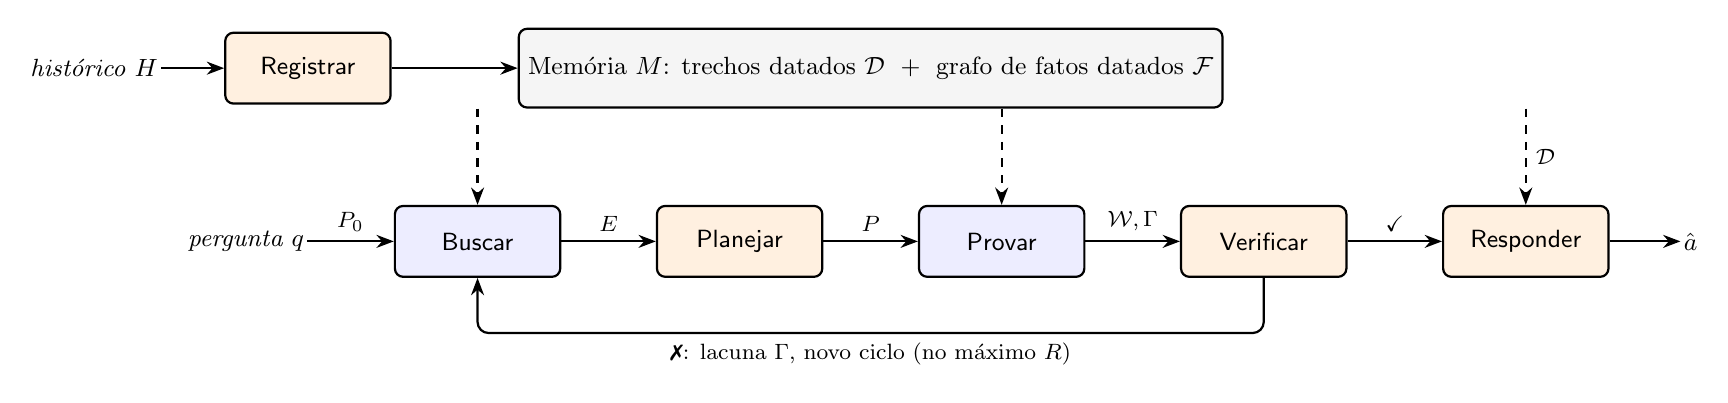
\begin{tikzpicture}[
  verb/.style={draw, rounded corners=3pt, thick, fill=blue!7, minimum
    height=9mm, minimum width=21mm, font=\sffamily\small},
  llm/.style={verb, fill=orange!12},
  obj/.style={font=\small\itshape, inner sep=1pt},
  arr/.style={-{Stealth[length=2.2mm]}, thick},
  lab/.style={font=\footnotesize, midway, above},
]
\node[obj] (q) at (0,0) {pergunta $q$};
\node[verb, right=11mm of q] (bus) {Buscar};
\node[llm, right=12mm of bus] (pla) {Planejar};
\node[verb, right=12mm of pla] (pro) {Provar};
\node[llm, right=12mm of pro] (ver) {Verificar};
\node[llm, right=12mm of ver] (res) {Responder};
\node[obj, right=9mm of res] (a) {$\hat a$};
\draw[arr] (q) -- node[lab]{$P_0$} (bus);
\draw[arr] (bus) -- node[lab]{$E$} (pla);
\draw[arr] (pla) -- node[lab]{$P$} (pro);
\draw[arr] (ver) -- node[lab]{\ok} (res);
\draw[arr] (res) -- (a);
\draw[arr] (pro) -- node[lab]{$\W,\Gamma$} (ver);
\draw[arr, rounded corners=4pt] (ver.south) -- ++(0,-7mm) -| node[pos=0.25, below,
  font=\footnotesize]{\ding{55}: lacuna $\Gamma$, novo ciclo (no máximo $R$)} (bus.south);
% memória
\node[draw, thick, rounded corners=3pt, fill=gray!8, minimum height=10mm,
  align=center, font=\small] (mem) at ($(pla)!0.5!(pro)+(0,2.2)$)
  {Memória $M$: trechos datados $\D$ \;+\; grafo de fatos datados $\F$};
\node[llm, left=16mm of mem] (reg) {Registrar};
\node[obj, left=8mm of reg] (h) {histórico $H$};
\draw[arr] (h) -- (reg);
\draw[arr] (reg) -- (mem);
\draw[arr, dashed] (mem.south -| bus) -- (bus.north);
\draw[arr, dashed] (mem.south -| pro) -- (pro.north);
\draw[arr, dashed] (mem.south -| res) -- node[right, font=\footnotesize]{$\D$} (res.north);
\end{tikzpicture}}
\caption{Fluxo do WitnessRAG. Componentes em laranja chamam o LLM; em azul,
não. \op{Registrar} roda uma vez por histórico. O ciclo
\op{Buscar}$\to$\op{Planejar}$\to$\op{Provar}$\to$\op{Verificar} termina
quando há prova e ela é confirmada (\ok) ou após $R$ ciclos. Sem prova,
\op{Verificar} devolve \ding{55} sem chamar o LLM, e a lacuna $\Gamma$ orienta
o próximo plano.}
\label{fig:fluxo}
\end{figure}

\begin{table}[H]
\centering
\small
\begin{tabularx}{\textwidth}{@{}l l Y l@{}}
\toprule
Componente & Assinatura & O que faz & LLM \\
\midrule
\op{Registrar} & $H\mapsto M$ & divide o histórico em trechos, extrai fatos, data tudo e grava a importância & sim, uma vez \\
\op{Buscar} & $(q,P,M)\mapsto E$ & acrescenta às evidências os $m$ trechos de maior pontuação $s_P$ & não \\
\op{Planejar} & $(q,E,\Gamma)\mapsto P$ & escreve a consulta, o tempo de referência e os pesos, vendo as evidências e a lacuna do ciclo anterior & sim \\
\op{Provar} & $(P,E,M)\mapsto(\W,\Gamma)$ & executa a consulta no grafo, das evidências para fora; devolve testemunhas e a lacuna & não \\
\op{Verificar} & $(q,P,\W)\mapsto\ok\mid\text{\ding{55}}$ & decide se o ciclo termina: confirma a prova ou a recusa & sim, se $\W\neq\varnothing$ \\
\op{Responder} & $(q,P,\W,M)\mapsto\hat a$ & escolhe $W^\ast$, resolve~\eqref{eq:objetivo} e lê o contexto & sim \\
\bottomrule
\end{tabularx}
\caption{Os seis componentes. \op{Registrar} fornece $\F(C)$, $\tau$ e
$\iota$; \op{Planejar} fixa $s_P$; \op{Buscar} fornece o material do plano;
\op{Provar} fornece as testemunhas; \op{Verificar} garante que elas respondem
a $q$; \op{Responder} resolve a Eq.~\eqref{eq:objetivo}. Só \op{Planejar}
escreve planos e só \op{Verificar} encerra o ciclo.}
\label{tab:componentes}
\end{table}

As duas camadas da memória correspondem a dois tipos de resultado. Na camada
de texto, trechos viram \emph{evidências} ($E$) e depois \emph{contexto}
($C$). Na camada lógica, fatos viram \emph{testemunha} ($W$) e a testemunha
aponta a resposta ($h(x)$). As camadas se ligam pela origem dos fatos:
$W\subseteq\F(C)$ diz que a prova está no texto que o leitor recebe.

% =====================================================================
\section{Registrar: a memória temporal}
\label{sec:registrar}

\paragraph{Trechos.} Turnos consecutivos são agrupados até $B$ tokens, sem
cortar turnos. A data do trecho é o intervalo das datas de sessão que ele
cobre, em geral um único dia.

\paragraph{Fatos.} Um LLM extrai fatos de cada janela de texto. Nomes que se
referem à mesma coisa (``Mel'' e ``Melanie'') são unidos em uma entidade
canônica de $\V$.

\paragraph{Três relógios.} Cada fato envolve três tempos: quando foi dito
($t_i$, a data da sessão), quando aconteceu ($\tau(f)$) e quando se pergunta
($t_q$). O tempo do evento é obtido normalizando a expressão temporal $e_f$ do
turno em relação à data em que foi dita:
\begin{equation}
\label{eq:tempo}
\tau(f)=
\begin{cases}
N(e_f,\,t_i) & \text{se o turno tem expressão temporal } e_f,\\
[t_i,t_i] & \text{caso contrário.}
\end{cases}
\end{equation}
Por exemplo, ``ontem'' dito em 8/5/2023 vira $[7/5,\,7/5]$ e ``semana
passada'' dito em 27/6/2023 vira $[19/6,\,25/6]$.

\paragraph{Importância.} Cada turno recebe na escrita uma nota
$\iota\in[0,1]$ que mede o quanto o falante marcou o evento como importante,
pela intensidade afetiva do texto~\citep{flexa2026bridging,mcgaugh2004amygdala}.
O fato herda a nota do turno de origem e o trecho recebe a maior nota entre os
seus turnos. A nota não depende da pergunta e é calculada uma única vez.

% =====================================================================
\section{Uma pontuação para toda a busca}
\label{sec:pontuacao}

Três sinais, todos em $[0,1]$, avaliam um item $x$ (trecho ou fato) em relação
a um alvo $y$. O alvo é a pergunta $q$ quando se ordenam trechos e é um átomo
$\alpha$ quando se ordenam fatos.

\begin{itemize}[leftmargin=*,itemsep=2pt]
\item \textbf{Similaridade} $\sigma(x,y)$. Para trechos, a fusão de uma busca
  densa com uma busca lexical, normalizada para $[0,1]$ sobre todos os trechos
  da memória.
  Para fatos, o grau em que $f$ instancia o átomo: relação e nomes.
\item \textbf{Importância} $\iota(x)$, gravada no \op{Registrar}.
\item \textbf{Proximidade temporal} ao tempo de referência do plano,
\begin{equation}
\label{eq:proximidade}
\rho_I(x)=\exp\!\Big(-\frac{\dist(\tau(x),I)}{\lambda_I}\Big),
\qquad
\lambda_I=
\begin{cases}
\max\{\lambda_0,\;|I|/2\} & \text{se } I \text{ é um período citado},\\
|H|/4 & \text{se } I=[t_q,t_q] \text{ ou } I=[t_1,t_1],
\end{cases}
\end{equation}
\end{itemize}

\noindent A pontuação é a combinação convexa dos três:
\begin{equation}
\label{eq:pontuacao}
\boxed{\;s_P(x\mid y)=w_\sigma\,\sigma(x,y)+w_\iota\,\iota(x)+w_\rho\,\rho_I(x)\;}
\end{equation}

\paragraph{Recência é proximidade a uma data.} A Eq.~\eqref{eq:proximidade}
cobre, com a mesma fórmula, as três buscas temporais que aparecem em
perguntas:
\begin{itemize}[leftmargin=*,itemsep=1pt]
\item $I=[t_q,t_q]$ (o agora): como todo item é anterior a $t_q$,
  $\rho=\exp(-(t_q-\tau^+)/\lambda_I)$, que cresce com a novidade. É a
  recência usual.
\item $I=[t_1,t_1]$ (o início do histórico): favorece o mais antigo, para
  perguntas como ``qual foi a primeira vez''.
\item $I$ um dia, mês ou ano citado na pergunta: $\rho=1$ dentro do período e
  decai fora dele; períodos com mais de $2\lambda_0$ dias decaem mais devagar.
\end{itemize}
Na ordenação, a data é \emph{suave}: um item fora do período perde pontuação,
mas não é descartado, o que protege contra erros de normalização de datas. No
corte de testemunhas (limiar $\theta$, Seção~\ref{sec:provar}), ela pesa na
medida de $w_\rho$: com $w_\rho$ alto, fatos longe de $I$ ficam abaixo do
corte. É o plano que decide o quanto a data restringe.

\paragraph{O plano regula os pesos.} O plano escolhe um nível por sinal
(nenhum, normal, forte). Calibrados sem LLM sobre o LoCoMo
(\texttt{docs/prova-v3-offline.md}), os níveis são: normal $=0$ para tempo e
importância, isto é, $w^0=(1,0,0)$; tempo forte $0{,}3$; importância forte
$0{,}1$; renormalizados para somar 1 com $w_\sigma\ge\frac12$. Com o período
``hoje'', qualquer peso não nulo mudou muitos contextos sem ganho de
revocação; com uma janela citada, o tempo forte elevou a revocação em todas as
categorias. A restrição $w_\sigma\ge\frac12$ tem uma consequência simples.

\begin{proposicao}[A similaridade manda]
\label{prop:sim}
Sejam $x$ um item sem relação com o alvo ($\sigma(x,y)=0$) e $x'$ um item
perfeitamente relacionado ($\sigma(x',y)=1$). Se $w_\sigma\ge\frac12$, então
$s_P(x\mid y)\le s_P(x'\mid y)$, por mais importante ou próximo no tempo que
$x$ seja; com $w_\sigma>\frac12$, a desigualdade é estrita.
\end{proposicao}
\begin{proof}
$s_P(x\mid y)\le w_\iota+w_\rho=1-w_\sigma\le w_\sigma\le s_P(x'\mid y)$,
e a segunda desigualdade é estrita quando $w_\sigma>\frac12$.
\end{proof}

\begin{proposicao}[Redução]
\label{prop:reducao}
Com $w=(1,0,0)$, $s_P=\sigma$ e toda ordenação do método coincide com a da
similaridade pura.
\end{proposicao}

% =====================================================================
\section{Buscar}
\label{sec:buscar}

\op{Buscar} acrescenta às evidências os $m$ trechos de maior pontuação sob o
plano corrente:
\begin{equation}
\label{eq:buscar}
E\;\leftarrow\;E\,\cup\,\Top_m\big(\D;\;s_P(\cdot\mid q)\big).
\end{equation}
A primeira busca usa o plano padrão $P_0$. As seguintes usam o plano do ciclo
anterior, que traz outro tempo de referência ou outros pesos e, com eles,
outros trechos: um plano com $I$ = junho de 2023 puxa os trechos de junho. As
evidências só crescem; nada encontrado antes se perde. Elas são o material de
trabalho de \op{Planejar} e \op{Provar}; o contexto final é escolhido sobre
toda a memória (Seção~\ref{sec:responder}).

% =====================================================================
\section{Planejar}
\label{sec:planejar}

\op{Planejar} é uma chamada ao LLM que recebe a pergunta \emph{e as
evidências}, com suas datas e os fatos $\F(E)$, e devolve
$P=(Q,\kappa,I,w)$. A partir do segundo ciclo recebe também a lacuna $\Gamma$
do ciclo anterior (Seção~\ref{sec:verificar}). Planejar depois de buscar
resolve três problemas de uma vez:
\begin{enumerate}[leftmargin=*,itemsep=1pt]
\item \emph{Vocabulário.} O planejador escreve relações e nomes como eles
  aparecem na memória, o que reduz a distância entre a consulta e os fatos.
\item \emph{Tempo.} Expressões da pergunta são resolvidas com $t_q$ e com as
  datas visíveis nas evidências, e viram o intervalo $I$.
\item \emph{Pesos.} O planejador vê se as evidências estão espalhadas no tempo
  ou concentradas, e ajusta $w$.
\end{enumerate}

O plano segue poucas regras, todas expressas na mesma linguagem:

\begin{table}[H]
\centering
\small
\begin{tabularx}{\textwidth}{@{}Y l l l@{}}
\toprule
Pergunta & Consulta $Q$ & $\kappa$ & $I$, $w$ \\
\midrule
Qual é a identidade de Caroline? & $Q(x)=\text{identidade}(\text{Caroline},x;\tau)$ & \um & padrão \\
Quando Caroline foi ao grupo de apoio? & $Q(\tau)=\text{foi\_a}(\text{Caroline},\text{grupo};\tau)$ & \um & padrão \\
Onde Melanie já acampou? & $Q(x)=\text{acampou\_em}(\text{Melanie},x;\tau)$ & \todos & padrão \\
Quando Melanie acampou em junho? & $Q(\tau)=\text{acampou\_em}(\text{Melanie},\_;\tau)$ & \um & junho, $w_\rho\uparrow$ \\
Qual foi a viagem mais recente de Jon? & $Q(x)=\text{viajou\_a}(\text{Jon},x;\tau)$ & \um & $[t_q,t_q]$, $w_\rho\uparrow$ \\
Onde mora a irmã de Ana? & $Q(z)=\text{irmã\_de}(y,\text{Ana};\tau_1)\wedge\text{mora\_em}(y,z;\tau_2)$ & \um & padrão \\
Caroline seguiria carreira de escritora? & $Q=\text{gosta\_de}(\text{Caroline},x;\tau_1)\wedge\text{objetivo}(\text{Caroline},y;\tau_2)$ & \todos & padrão \\
\bottomrule
\end{tabularx}
\caption{Exemplos de planos. Perguntas simples têm um átomo; ``quando''
torna o tempo a variável de resposta; datas e ``mais recente'' viram $I$;
perguntas de conjunto usam $\kappa=\todos$; em perguntas inferenciais, os
átomos são as premissas de que o leitor precisa. O símbolo $\_$ é uma variável
existencial.}
\label{tab:planos}
\end{table}

% =====================================================================
\section{Provar}
\label{sec:provar}

\op{Provar} executa a consulta no grafo de fatos. Não chama o LLM.

\paragraph{Compilação.} Os átomos são ordenados de modo que cada um, a partir
do segundo, compartilhe uma variável com os anteriores, começando pelo que tem
mais nomes fixos. Cada átomo $\alpha_j$ admite os candidatos
$A_j(\F')=\{f\in\F':\sigma(f,\alpha_j)\ge\theta_\alpha\}$.

\paragraph{Exploração de caminhos.} Como átomos consecutivos compartilham
variáveis, um casamento é um caminho no grafo. A exploração é uma busca em
feixe de largura $b$:
\begin{equation}
\label{eq:feixe}
B_0=\{\varnothing\},\qquad
B_j=\Top_b\big\{\,h\cup\{\alpha_j\mapsto f\}\;:\;h\in B_{j-1},\;f\in A_j(\F'),\;
\text{consistente}\,\big\},
\end{equation}
ordenada pela pontuação do caminho, a média geométrica da
Eq.~\eqref{eq:pontuacao} ao longo dos passos:
\begin{equation}
\label{eq:caminho}
S_P(h)=\Big(\prod_{\alpha\in\mathrm{dom}(h)}s_P\big(h(\alpha)\mid\alpha\big)\Big)^{1/|h|}.
\end{equation}
Assim, cada passo da exploração leva em conta a similaridade com o átomo, a
importância do fato e a proximidade ao tempo de referência, com os pesos do
plano. As testemunhas são os caminhos completos com pontuação suficiente,
$\W(\F')=\{h(Q):h\in B_L,\;S_P(h)\ge\theta\}$.

\paragraph{Limiar.} Todo fato admissível tem $s_P\ge w_\sigma\theta_\alpha$, logo
todo casamento tem $S_P\ge w_\sigma\theta_\alpha$. O limiar só filtra algo
quando $\theta>w_\sigma\theta_\alpha$, e é nessa faixa que ele é calibrado.

\paragraph{Evidências primeiro.} A prova é procurada primeiro dentro das
evidências e só depois no grafo inteiro:
\begin{equation}
\label{eq:provar}
\W=
\begin{cases}
\W(\F(E)) & \text{se } \kappa=\um \text{ e } \W(\F(E))\neq\varnothing,\\
\W(\F) & \text{caso contrário.}
\end{cases}
\end{equation}
Uma prova dentro das evidências é a mais segura, porque o planejador leu esses
trechos ao escrever o plano. Só quando as evidências não contêm a prova a
exploração sai delas e percorre o grafo pelos caminhos que a consulta
determina. Para $\kappa=\todos$ a busca no grafo inteiro sempre acontece: não
se certifica que um conjunto está completo olhando só parte da memória.

\paragraph{Lacuna.} Sem testemunha, \op{Provar} devolve a lacuna $\Gamma$: os
átomos sem nenhum candidato ($A_j(\F)=\varnothing$) e o átomo em que o feixe
esvaziou (o primeiro $j$ com $B_j=\varnothing$). Com testemunha,
$\Gamma=\varnothing$.

\paragraph{Plano completo.} O plano está completo quando existe prova:
\begin{equation}
\label{eq:parada}
\mathrm{completo}(P)\iff\W\neq\varnothing.
\end{equation}
Com $\kappa=\um$, se as evidências já contêm uma testemunha, o plano se
completa sem sair delas.

% =====================================================================
\section{Verificar}
\label{sec:verificar}

\op{Verificar} é o único componente que encerra o ciclo:
\begin{equation}
\label{eq:verificar}
v=
\begin{cases}
\text{\ding{55}} & \text{se } \W=\varnothing,\\
\op{Confirma}(q,P,\W)\in\{\ok,\text{\ding{55}}\} & \text{caso contrário.}
\end{cases}
\end{equation}
Sem prova, a resposta é \ding{55} e não há chamada ao LLM. Se a prova
escolhida já está no contexto ($D(W^\ast)\subseteq\Top_k(\D;s_P)$), a
resposta é \ok{} sem chamada: confirmar não mudaria o contexto. Nos demais
casos, uma chamada lê cada resposta candidata com os seus fatos datados e a
fala de origem de cada fato, e confirma ou recusa cada uma; uma recusa exige
entidade, período ou tipo errados, ou falta de suporte, e o motivo entra na
lacuna $\Gamma$. A verificação confirma; não procura.

O ciclo termina quando $v=\ok$, isto é, quando o plano está completo
(Eq.~\eqref{eq:parada}) e a prova é confirmada, ou após $R$ ciclos. Caso
contrário, o próximo ciclo busca com o plano atual e \op{Planejar} escreve um
novo plano que ataca a causa da lacuna: o nome da relação, um nome próprio, o
tempo de referência, os pesos ou $\kappa$. O papel lembra a autorreflexão do
Reflexion~\citep{shinn2023reflexion}, com uma diferença: a lacuna é objetiva
(qual átomo falhou ou por que a prova foi recusada), e não um diagnóstico
livre.

% =====================================================================
\section{Responder}
\label{sec:responder}

\paragraph{Escolha das testemunhas.} Só se usa prova confirmada: se o último
ciclo terminou com \ding{55}, $W^\ast=\varnothing$. Caso contrário, as
testemunhas são percorridas em ordem decrescente de $S_P$ (com desempate fixo)
e acumuladas em $W^\ast$: apenas a primeira quando $\kappa=\um$, todas as que
couberem quando $\kappa=\todos$. Uma testemunha $W$ entra se, com ela,
\begin{equation}
\label{eq:escolha}
|D(W^\ast\cup W)|\le k
\qquad\text{e}\qquad
|D(W^\ast\cup W)\setminus\Top_k(\D;s_P)|\le k_W .
\end{equation}
A primeira condição garante que a prova cabe no contexto; a segunda limita
quantos trechos ela pode trazer de fora dos $k$ melhores. Testemunhas cujos
trechos já estão entre os $k$ melhores não gastam nada desse limite. Usamos
$k_W=2$ para um plano composto (átomos conectados ou $\kappa=\todos$) e
$k_W=1$ para um plano de um átomo com $\kappa=\um$. Uma testemunha só é
utilizável se a busca foi seletiva (até 3 respostas e 3 testemunhas, sem
cortes) e se o seu casamento bruto, $\prod_j\sigma(h(\alpha_j),\alpha_j)$
vezes a confiança dos fatos, passa de $\theta$; os pesos do plano ordenam as
testemunhas, mas não decidem se uma vale.

\paragraph{Contexto.} A solução da Eq.~\eqref{eq:objetivo} é direta:
\begin{equation}
\label{eq:contexto}
C^\ast=D(W^\ast)\;\cup\;\Top_{k-|D(W^\ast)|}\big(\D\setminus D(W^\ast);\;s_P(\cdot\mid q)\big).
\end{equation}

\begin{proposicao}[Seleção exata]
\label{prop:exata}
Dado $W^\ast$ com $|D(W^\ast)|\le k$, a Eq.~\eqref{eq:contexto} resolve a
Eq.~\eqref{eq:objetivo} exatamente.
\end{proposicao}
\begin{proof}
A restrição $W^\ast\subseteq\F(C)$ equivale a $D(W^\ast)\subseteq C$. O
objetivo é uma soma de pontuações individuais sob limite de cardinalidade;
fixados os trechos obrigatórios, as vagas restantes ficam com as maiores
pontuações.
\end{proof}

O leitor recebe os trechos com suas datas, os da testemunha por último, mais
perto da pergunta, e escreve $\hat a=\op{Leitor}(q,C^\ast)$. A testemunha já
aponta $h(x)$; o leitor dá a forma final e faz a aritmética de datas quando a
pergunta pede. Sem prova confirmada, \eqref{eq:contexto} se reduz a
$\Top_k(\D;s_P)$.

% =====================================================================
\section{Algoritmo, custo e garantias}

\begin{algorithm}[H]
\caption{WitnessRAG para uma pergunta}
\label{alg:witnessrag}
\begin{algorithmic}[1]
\Require pergunta $q$, memória $M=(\D,\F,\V)$, orçamento $k$, ciclos $R$
\State $E\gets\varnothing$;\; $P\gets P_0$;\; $\Gamma\gets\varnothing$
\For{$r=1,\dots,R$}
  \State $E\gets E\cup\Top_m(\D;\,s_P(\cdot\mid q))$ \Comment{Buscar, Eq.~\eqref{eq:buscar}}
  \State $P\gets\op{Planejar}(q,E,\Gamma)$ \Comment{$\Gamma=\varnothing$ no primeiro ciclo}
  \State $(\W,\Gamma)\gets\op{Provar}(P,E,M)$ \Comment{Eqs.~\eqref{eq:feixe}--\eqref{eq:parada}}
  \State $v\gets\op{Verificar}(q,P,\W)$ \Comment{sem LLM se $\W=\varnothing$}
  \If{$v=\ok$} \textbf{break} \EndIf
  \State $\Gamma\gets\Gamma\cup\{\text{motivo de } v\}$
\EndFor
\State $W^\ast\gets$ testemunhas de $\W$ escolhidas pela Eq.~\eqref{eq:escolha} se $v=\ok$; senão $\varnothing$
\State $C^\ast\gets D(W^\ast)\cup\Top_{k-|D(W^\ast)|}(\D\setminus D(W^\ast);\,s_P)$ \Comment{Eq.~\eqref{eq:contexto}}
\State \Return $\op{Leitor}(q,C^\ast)$
\end{algorithmic}
\end{algorithm}

\paragraph{Custo.} Cada ciclo faz uma chamada de \op{Planejar} e, se houver
prova, uma de \op{Verificar}; a leitura é uma chamada. Com $r$ ciclos, dos
quais $r_W\le r$ encontraram prova, são $r+r_W+1$ chamadas: três quando o
primeiro ciclo termina confirmado e no máximo $2R+1$. \op{Buscar} e
\op{Provar} não chamam o LLM. \op{Registrar} roda uma vez por histórico.

\paragraph{Garantias.}
\begin{proposicao}[Suficiência]
Se $W^\ast\neq\varnothing$, então $W^\ast\subseteq\F(C^\ast)$: todas as
premissas da resposta, com suas datas, estão no contexto do leitor.
\end{proposicao}

\begin{proposicao}[Mudança limitada]
\label{prop:limitada}
$|C^\ast\setminus\Top_k(\D;s_P)|\le k_W$: a prova troca no máximo $k_W$
trechos do contexto que se teria sem ela.
\end{proposicao}
\begin{proof}
Seja $D=D(W^\ast)$. Com desempate fixo, um trecho entre os $k-|D|$ melhores de
$\D\setminus D$ tem acima de si no máximo $k-|D|-1$ trechos de $\D\setminus D$
e $|D|$ trechos de $D$, logo está em $\Top_k(\D)$. Os trechos de $C^\ast$ fora
de $\Top_k(\D)$ estão, portanto, em $D\setminus\Top_k(\D)$, cujo tamanho é
limitado por $k_W$ na Eq.~\eqref{eq:escolha}.
\end{proof}

\begin{proposicao}[A linha de base está contida]
Com $w=(1,0,0)$ em todos os planos e sem prova confirmada,
$C^\ast=\Top_k(\D;\sigma)$, a recuperação por similaridade. Cada ablação do
método é um ponto desse espaço de desenho.
\end{proposicao}

% =====================================================================
\section{Três perguntas do LoCoMo}
\label{sec:exemplos}

Os exemplos usam turnos reais da primeira conversa do
LoCoMo~\citep{maharana2024locomo}. São ilustrativos: a divisão em trechos e os
fatos extraídos dependem da execução.

\paragraph{A. A prova já está nas evidências.} \emph{``When did Caroline go
to the LGBTQ support group?''} (ouro: 7 May 2023).
\begin{itemize}[leftmargin=*,itemsep=1pt]
\item \op{Registrar}: o turno D1:3, da sessão de 8/5/2023, diz ``I went to a
  LGBTQ support group yesterday''. Pela Eq.~\eqref{eq:tempo},
  $f_1=(\text{Caroline},\text{foi\_a},\text{grupo LGBTQ},[7/5/2023],d_1)$.
\item \op{Buscar} com $P_0$ traz $d_1$, que é muito similar à pergunta.
\item \op{Planejar}: $Q(\tau)=\text{foi\_a}(\text{Caroline},\text{grupo LGBTQ};\tau)$,
  $\kappa=\um$, $I$ e $w$ padrão.
\item \op{Provar}: $f_1\in\F(E)$, então $\W=\{\{f_1\}\}$ sem sair das
  evidências. O plano está completo.
\item \op{Verificar} confirma e o leitor responde ``7 May 2023''. Três
  chamadas: planejar, verificar e ler.
\end{itemize}

\paragraph{B. A prova sai das evidências.} \emph{``Where has Melanie
camped?''} (ouro: beach, mountains, forest; turnos D4:6, D6:16 e D8:32, das
sessões de 27/6, 6/7 e 15/7/2023).
\begin{itemize}[leftmargin=*,itemsep=1pt]
\item \op{Planejar}: $Q(x)=\text{acampou\_em}(\text{Melanie},x;\tau)$,
  $\kappa=\todos$.
\item \op{Provar}: como $\kappa=\todos$, a busca vai ao grafo inteiro e
  encontra três testemunhas de um fato cada, em três sessões diferentes.
\item \op{Verificar} confirma o conjunto. Suponha que os trechos de 27/6 e 6/7
  já estejam entre os $k$ melhores por $s_P$: o de 15/7 entra no contexto e
  desloca um único trecho, dentro do limite $k_W=2$
  (Proposição~\ref{prop:limitada}). O leitor responde ``beach, mountains,
  forest''.
\end{itemize}

\paragraph{C. Busca por data.} \emph{``When did Melanie go camping in
June?''} (ouro: the week before 27 June 2023).
\begin{itemize}[leftmargin=*,itemsep=1pt]
\item \op{Planejar}: $Q(\tau)=\text{acampou\_em}(\text{Melanie},\_;\tau)$,
  $\kappa=\um$, $I=[1/6,\,30/6/2023]$, $w=(0{,}7;\;0;\;0{,}3)$ (tempo forte).
\item Os fatos candidatos têm tempos $[19/6,25/6]$ (montanhas: ``last week''
  dito na terça, 27/6, com semanas de segunda a domingo), $[6/7,6/7]$
  (praia), $[8/7,9/7]$ (``two weekends ago'' dito em 17/7) e
  $[15/7,15/7]$ (floresta). Com $\lambda_I=\max\{7,\,30/2\}=15$ dias, as
  distâncias a junho são $0$, $6$, $8$ e $15$ dias e a
  Eq.~\eqref{eq:proximidade} dá $\rho=1$; $0{,}67$; $0{,}59$ e $0{,}37$.
\item Com similaridades iguais, as pontuações diferem apenas pela parcela do
  tempo, $w_\rho\,\rho$: $0{,}30$; $0{,}20$; $0{,}18$ e $0{,}11$. A viagem de
  junho vence, e a testemunha dá $\tau=[19/6,25/6]$: ``a semana antes de 27 de
  junho''. É a recência tomada em relação a junho, e não ao agora.
\item O turno D2:7 (``thinking about going camping next month'', dito em
  25/5) também cai em junho, mas é um plano, não um acontecimento: o fato
  extraído tem outra relação (\emph{planeja acampar}) e perde na similaridade
  com o átomo.
\end{itemize}

% =====================================================================
\section{Desenho experimental}

\paragraph{Protocolo.} Seguimos o protocolo do GAM~\citep{yan2025gam}: LoCoMo
como avaliação principal (F1 e BLEU-1 por categoria, 1.540 perguntas, sem as
adversariais), HotpotQA com 56K, 224K e 448K
tokens~\citep{yang2018hotpotqa}, RULER 128K~\citep{hsieh2024ruler} e
NarrativeQA~\citep{kocisky2018narrativeqa}. Leitor, modelo de
embeddings~\citep{chen2024bgem3}, tamanho de trecho ($B=2048$) e orçamento
($k=5$) são os mesmos para todos os métodos.

\paragraph{Linhas de base.} Recuperação híbrida (densa + lexical com
RRF~\citep{cormack2009rrf}), GraphRAG~\citep{edge2024graphrag},
HippoRAG 2~\citep{gutierrez2025hipporag2}, GAM, Zero-Mem e um executor
relacional sobre os \emph{mesmos} fatos, sem critério de testemunha, que
isola a contribuição da prova da contribuição da extração.

\paragraph{Perguntas de pesquisa.}
\begin{enumerate}[label=\textbf{Q\arabic*},leftmargin=*,itemsep=1pt]
\item \emph{Prova como critério.} Selecionar o contexto sob restrição de
  prova melhora a resposta em relação às linhas de base, em cada categoria?
\item \emph{Planejar depois de buscar.} Um plano escrito com as evidências é
  melhor do que um plano escrito só com a pergunta?
\item \emph{Pesos pelo plano.} Pesos definidos pelo planejador superam pesos
  fixos? Qual é o efeito de $\iota$ e de $\rho$, em especial nas perguntas
  temporais?
\item \emph{Parada e custo.} Com que frequência a prova já está nas
  evidências iniciais ($r=1$)? Quantas chamadas e tokens o método gasta por
  pergunta, comparado ao GAM?
\end{enumerate}

\begin{table}[H]
\centering
\small
\begin{tabularx}{\textwidth}{@{}l Y l@{}}
\toprule
Variante & O que muda & Pergunta \\
\midrule
Similaridade pura & $w=(1,0,0)$, sem plano nem prova & base \\
Sem prova & plano e pesos, mas $W^\ast=\varnothing$ sempre & Q1 \\
Plano cego & \op{Planejar}$(q)$, sem ver $E$ & Q2 \\
Pesos fixos & $w=w^0$ sempre & Q3 \\
Sem importância / sem tempo & $w_\iota=0$ / $w_\rho=0$ & Q3 \\
Sem evidências primeiro & \op{Provar} sempre no grafo inteiro & Q4 \\
Verificação fundida & \op{Verificar} e \op{Responder} na mesma chamada & Q4 \\
\bottomrule
\end{tabularx}
\caption{Ablações. Cada linha muda uma única decisão do método.}
\label{tab:ablacoes}
\end{table}

\paragraph{Hiperparâmetros.} Valores usados na implementação:
$B=2048$ tokens, $k=5$, $m=20$, $k_W=2$ (plano composto) e $1$ (plano
simples), $b=400$, $\theta_\alpha=0{,}65$, $\theta=0{,}45$ sobre o casamento
bruto, $\lambda_0=7$ dias, $\lambda_I=|H|/4$ para o agora e o início, $R=2$;
níveis de peso: normal $w^0=(1,0,0)$, tempo forte $0{,}3$, importância forte
$0{,}1$.

% =====================================================================
\appendix
\section{Implementação}

O desenho está implementado como a opção \texttt{-{}-proof-controller}, no
método \texttt{\_retrieve\_proof} de \texttt{wrag/\allowbreak methods/\allowbreak
witnessrag.py}. A tabela liga cada objeto da formulação ao código.

\begin{table}[H]
\centering
\small
\begin{tabularx}{\textwidth}{@{}l Y@{}}
\toprule
Objeto & Código \\
\midrule
$\tau(d)$, $\tau(f)$, $\iota$, fala de origem & \texttt{witness/dated\_memory.py} (Eq.~\eqref{eq:tempo}, com \texttt{timeline.resolve\_expression}) \\
$s_P$, $\rho_I$, níveis de $w$ & \texttt{witness/scoring.py} \\
$P=(Q,\kappa,I,w)$ & \texttt{witness/plan.py}; o átomo ganhou um espaço de tempo para respostas ``quando'' \\
Casamento, feixe, $S_P$ & \texttt{witness/search.py} (prior $w_\iota\iota+w_\rho\rho$ somado a $w_\sigma\sigma$ em cada passo; casamento bruto guardado para o limiar) \\
\op{Verificar} & \texttt{witness/confirm.py} \\
Eq.~\eqref{eq:contexto}, $k_W$ & \texttt{methods/witnessrag.py} \\
\bottomrule
\end{tabularx}
\caption{Da formulação ao código.}
\label{tab:mapa}
\end{table}

\bibliographystyle{plainnat}
\bibliography{witnessrag}

\end{document}
